\section{Kecerdasan Buatan}
\subsection{Definisi Kecerdasan Buatan}
 \hspace{1cm} Kecerdasan  buatan  (Arificial  Intellegence/AI) merupakan   perkembangan   teknologi   informasi   dan komunikasi  yang  mengemuka  dalam  sepuluh  tahun terakhir.  Pemanfaatan  AI  oleh  industri  tidak  hanya terbatas di sektor industri telekomunikasi, namun juga di sektor perbankan, manufaktur, jasa, bahkan di sektor pemerintah.    Dibeberapa negara, implementasi kecerdasan   buatan   sudah   mencapai   hampir 56 persen,terutama  pada  sektor  industri. Namun   implementasi   AI   di Indonesia    tergolong   rendah, karena banyaknya permasalahan seperti skill pekerja yang belum memenuhi  untuk  mengoperasikan  AI  serta  kurangnya investasi   untuk   mengembangkan   infrastruktur   AI. Beberapa  penelitian  terdahulu  menyimpulkan  bahwa penyerapan   teknologi di Indonesia lebih rendah dibandingkan kawasan Asia Pasifiklainnya. Hanya 14 perusahaan di Indonesia yang telah mengadopsi teknologi berbasis AI. Ada 6 faktor utama yang  menentukan  keberhasilan implementasi  AI  yaitu kepemimpinan,kemampuan berfikir analisis dan sistematis,budaya  perusahaan, inisiatif, manajemen, dan kewirausahaan.
 
\hspace{1cm}Contoh  implementasi  AI  sebagai  penggunaan teknologi informasi adalah cloud computing yang disajikan berdasarkan utilitas secara on demand.Cloud computing sebenarnya  bukanlah  hal  yang  baru  dalam dunia   teknologi informasi. Web   service, internet service provider(ISP), programmable web,   dan virtualisasi   merupakan   konsep-konsep   yang   telah berkembang   dan   memberi   kontribusi   pada   evolusi teknologi ini. Beberapa definisi mengenai konsep cloud computingtelah   sering   dikemukakan   diberbagai literatur.

\hspace{1cm} Menurut John McCarthy(1956) Kecerdasan buatan adalah usaha memodelkan proses berpikir manusia dan mendesain mesin agar dapat menirukan perilaku manusia. dan masih banyak lagi ahli pendapat mengenai definisi dari kecerdasan buatan. namun kembali lagi pada secercah ceritita diatas, poin utamanya adalah bagaimana manusia menciptakan teknologi yang mampu berpikir seperti manusia itu sendiri itulah sederhananya definisi kecerdasan buatan atau dalam bahasa inggris Artificial Intellegent atau AI. Perusahaan di Indonesia pada umumnya masih membeli dan menggunakan server sendiri untuk kebutuhan bisnisnya. Kondisi  ini  menunjukkan cloud  computing memiliki peluang yang besar untuk meningkatkan performa perusahaan.    Namun  Indonesia  masih terkendala  pada  masalah keterbatasan bandwidth, dimana  hal  ini  merupakan  masalah  yang  besar  untuk menyambut cloud   computing masuk   ke   tanah   air. Karakteristiknya yang bersifat on demand akan sangat bergantung pada kualitas jaringan internet yang memadai  demi  penyampaian layanan   yang handal. Namun  hal  ini  dapat  disiasati dengan penggunaan layanan cloudyang  ringan  dan  inovasi  yang terus-menerus. Bercermin dari kondisi saat ini, Kementerian Komunikasi  dan  Informatika  RI  menyatakan  bahwa diperkirakan Indonesia  masih  memerlukan waktu 3-5 tahun  lagi untuk  mengadopsi  teknologi  ini untuk    meningkatkan   pengembangan open government, banyak  instansi  yang membutuhkan Big Data Processing termasuk High Performance Computing(HPC). Beberapa  penelitian  menyatakan bahwa HPC  telah membuka batas baru dalam memecahkan  masalah  teknik  struktural  skala  besar. Beberapa tinjauan artikel menyatakan bahwa HPC saat ini  berkembang  di Asia khususnya  Asia  Tenggara.

\subsection{Sejarah dan perkembangan Kecerdasan Buatan}
\hspace{1cm} Kecerdasan buatan merupakan bidang ilmu komputer yang sangat penting di era kini dan masa akan datang untuk mewujudkan sistem komputer yang cerdas.  Bidang ini telah berkembang sangat pesat di 20 tahun terakhir seiring dengan kebutuhan perangkat cerdas pada industry dan rumah tangga, oleh karena itu buku ini memaparkan berbagai pandangan modern dan hasil riset terkini  yang perlu dikuasai oleh para akademisi, pelajar dan praktisi lengkap dengan implementasi nyata.

\hspace{1cm} Kata “intelligence” berasal dari bahasa Latin “intelligo” ang bearti “saya paham”.  Barti dasar dari intelligence ialah kemampuan untuk memahami dan melakukan aksi.  Sebenarnya, area Kecerdasan Buatan (Artificial Intelligence) atau disingkat dengan AI,  bermula dari kemunculan komputer sekitar th 1940-an, meskipun sejarah perkembangannya dapat dilacak sejak zaman Mesir kuno. Pada masa ini, perhatian difokuskan pada kemampuan komputer mengerjakan sesuatu yang dapat dilakukan oleh manusia.  Dalam hal ini, komputer tersebut dapat meniru kemampuan kecerdasan  dan perilaku  manusia

\hspace{1cm} McMulloh dan Pitts pada tahun 1943 mengusulkan model matematis bernama perceptron dari neuron di dalam  otak.  Mereka juga menunjukkan  bagaimana neuron menjadi aktif seperti saklar on-off dan neuron tersebut mampu untuk belajar dan memberikan aksi berbeda terhadap waktu dari input yang diberikan.  Sumbangan terbesar di bidang AI diawali pada paper Alan Turing, pada tahun 1950 yang mencoba menjawab  “Dapatkah computer berfikir” dengan menciptakan mesin Turing.  Paper Alan Turing pada tahun 1950 berjudul “Computing Machineri and Intelligence” mendiskusikan syarat sebuah mesin dianggap cerdas. Dia beranggapan bahwa jika mesin dapat dengan sukses berprilaku seperti manusia, kita dapat menganggapnya cerdas.

\hspace{1cm} Pada akhir 1955, Newell dan Simon mengembangkan  The Logic Theorist, program AI pertama. Program ini merepresentasikan  masalah sebagai model pohon, lalu penyelesaiannya dengan  memilih cabang yang akan menghasilkan kesimpulan terbenar. Program ini berdampak besar dan menjadi batu loncatan penting dalam mengembangkan bidang AI. Pada tahun 1956 John McCarthy dari  Massacuhetts Institute of Technology dianggap sebagai bapak AI, menyelenggarakan konferensi untuk menarik para ahli komputer bertemu, dengan  nama kegiatan “The Dartmouth summer research project on artificial intelligence.” 

\hspace{1cm} Pada  tahun 1960 hingga 1970, muncul berbagai dikusi bagaimana komputer dapat meniru sedetail mungkin pada kemampuan otak manusia, dimana saat itu dapat dikategorikan sebagai “classical AI”. Pada tahun 1980, dimana computer yang semakin mudah diperoleh dengan harga yang lebih murah menjadikan berbagai riset di bidang kecerdasan buatan berkembang sangat pesat pada berbagai universitas.  Tabel 1.1 merupakan rangkuman sejarah penting pengembagan bidang Kecerdasan Buatan.

\subsection{Supervised learning dan Unsupervised Learning}
\hspace{1cm} Berbicara mengenai AI , didalam AI adapun yang disebut dengan Machine learning dimana akan dikategorikan berdasarkan label atau tag. Maksud dari tag atau label ini adalah lebih membahas tentang target variable apakah ada atau tidak dasar datanya. 
 
\hspace{1cm} Supervised Learning merupakan proses pengelompokan data yang telah memiliki label dan akan dikelompokkan berdasarkan labelnya. Untuk mendapatkan label tentunya harus melakukan proses training terlebih dahulu. Contohnya, kita memiliki 3 kriteria dengan skalanya masing masing. Misalkan Suhu tinggi (1), batuk (0), sesak napas (0) maka corona (0), dimana angka 1 menunjukkan “ya” dan angka 0 menujukkan “tidak”.

\hspace{1cm} Sedangkan Unsupervised Learning merupakan proses pengelompokan data yang tidak memiliki label. Sehingga kita bebas menentukan berapa jumlah kelompok data yang akan dibuat, misalnya menjadi 2, 3 atau seterusnya. Tentunya dalam pengelompokan ini juga berdasarkan karakteristiknya yang sama. Nah, untuk outputnya sendiri tentunya akan berbeda dengan supervised learning. Karena outputnya belum diketahui, maka kita dapat membuatnya sendiri dengan mengelompokkannya.

\subsection{Data Set, Training Test, Testing Test}
\hspace{1cm} Berbicara mengenai Supervised learning serta unsupervised learning maka harus adanya pembahasan mengenai definisi dataset. Dataset adalah kumpulan sampel yang sudah dikumpulkan. Seorang anak ingin bermain badminton, tetapi keputusannya untuk bermain badminton (play) tergantung pada variable yang ditentukan contohnya jarak kaki dari gairs dan atau tinggi net sehingga variable varibale ini disebut fitur.

\hspace{1cm} Sedangkan Training set adalah bagian dataset yang kita latih untuk membuat prediksi atau menjalankan fungsi dari sebuah algoritma ML. Kita memberikan petunjuk melalui algoritma agar mesin yang kita latih bisa mencari korelasinya sendiri atau belajar pola dari data yang diberikan.Testing Test adalah bagian dataset yang kita tes untuk melihat keakuratannya, atau dengan kata lain melihat performanya.


\section{Instalasi}
\begin{enumerate}
    \item Instalasi library scikit dari anaconda dengan pip install -U scikit-learn
     \begin{center}
    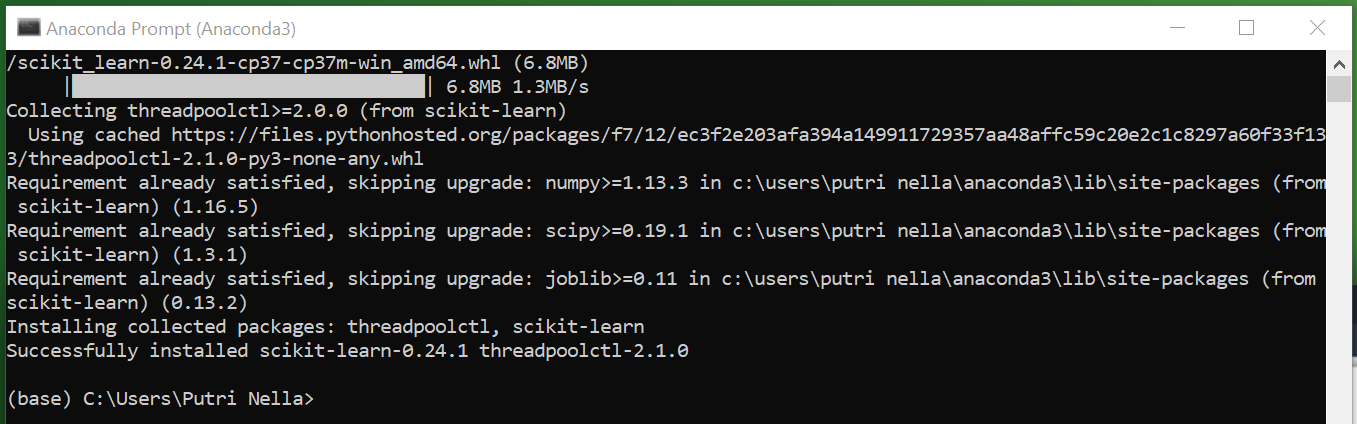
\includegraphics[width=.8\textwidth]{figures/1184017/chapter1/1.PNG}
    \end{center}
    \item Mencoba Loading dan example dataset.
    \begin{center}
    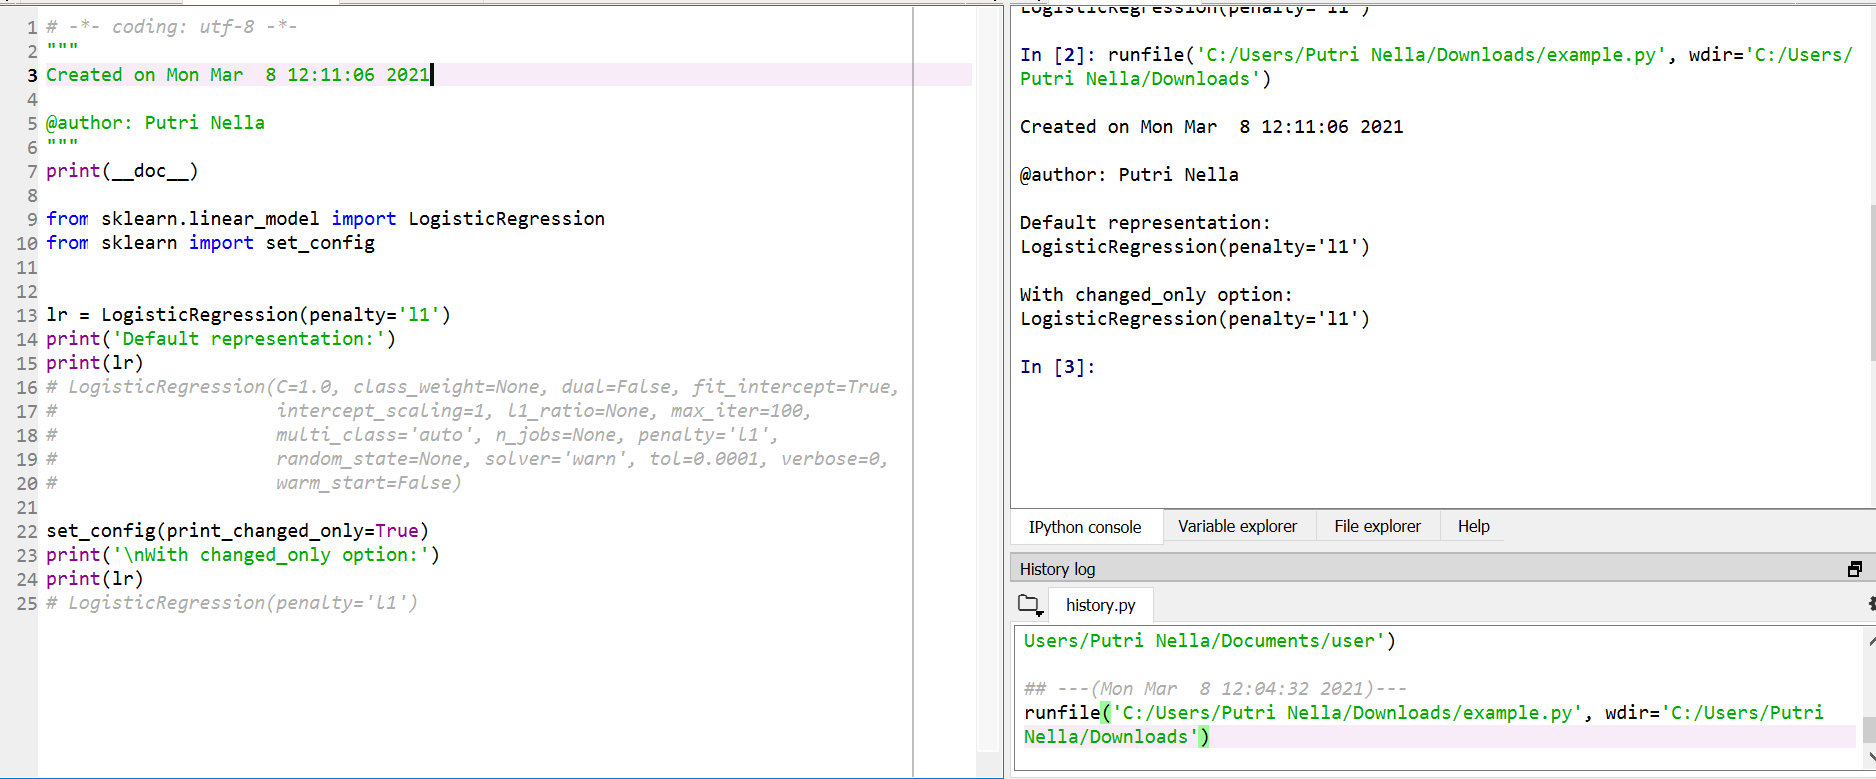
\includegraphics[width=.8\textwidth]{figures/1184017/chapter1/2.PNG}
    \end{center}
     \begin{center}
    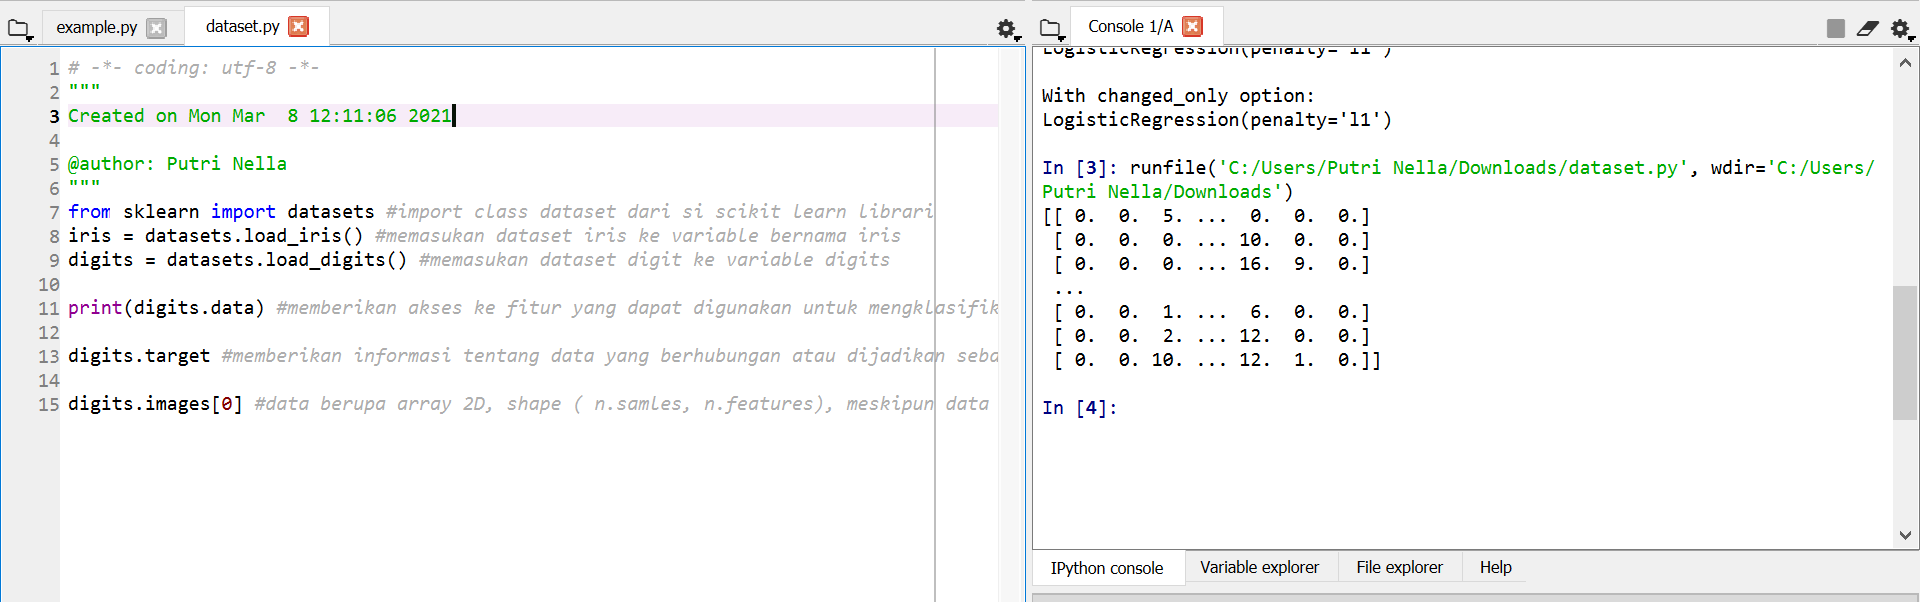
\includegraphics[width=.8\textwidth]{figures/1184017/chapter1/3.PNG}
    \end{center}
    \item Mencoba Learning and predicting.
    \begin{center}
    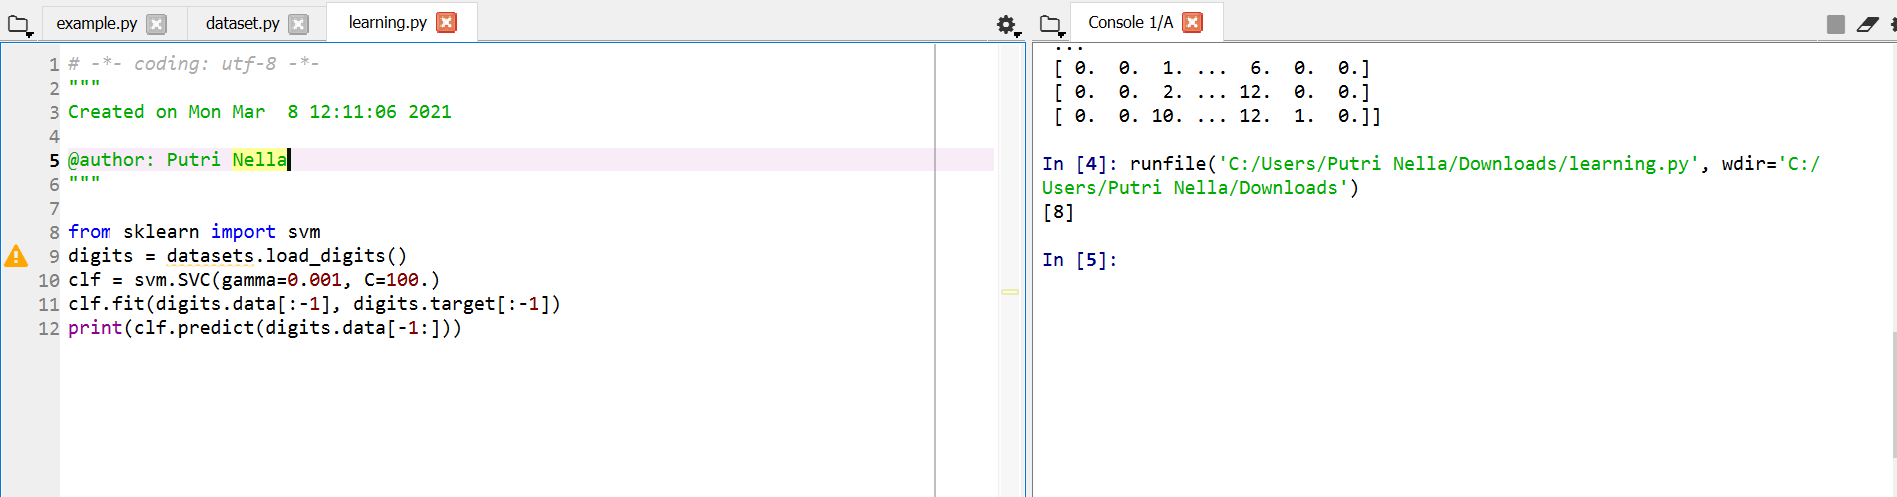
\includegraphics[width=.8\textwidth]{figures/1184017/chapter1/4.PNG}
    \end{center}
    \item Mencoba Model persistence
    \begin{center}
    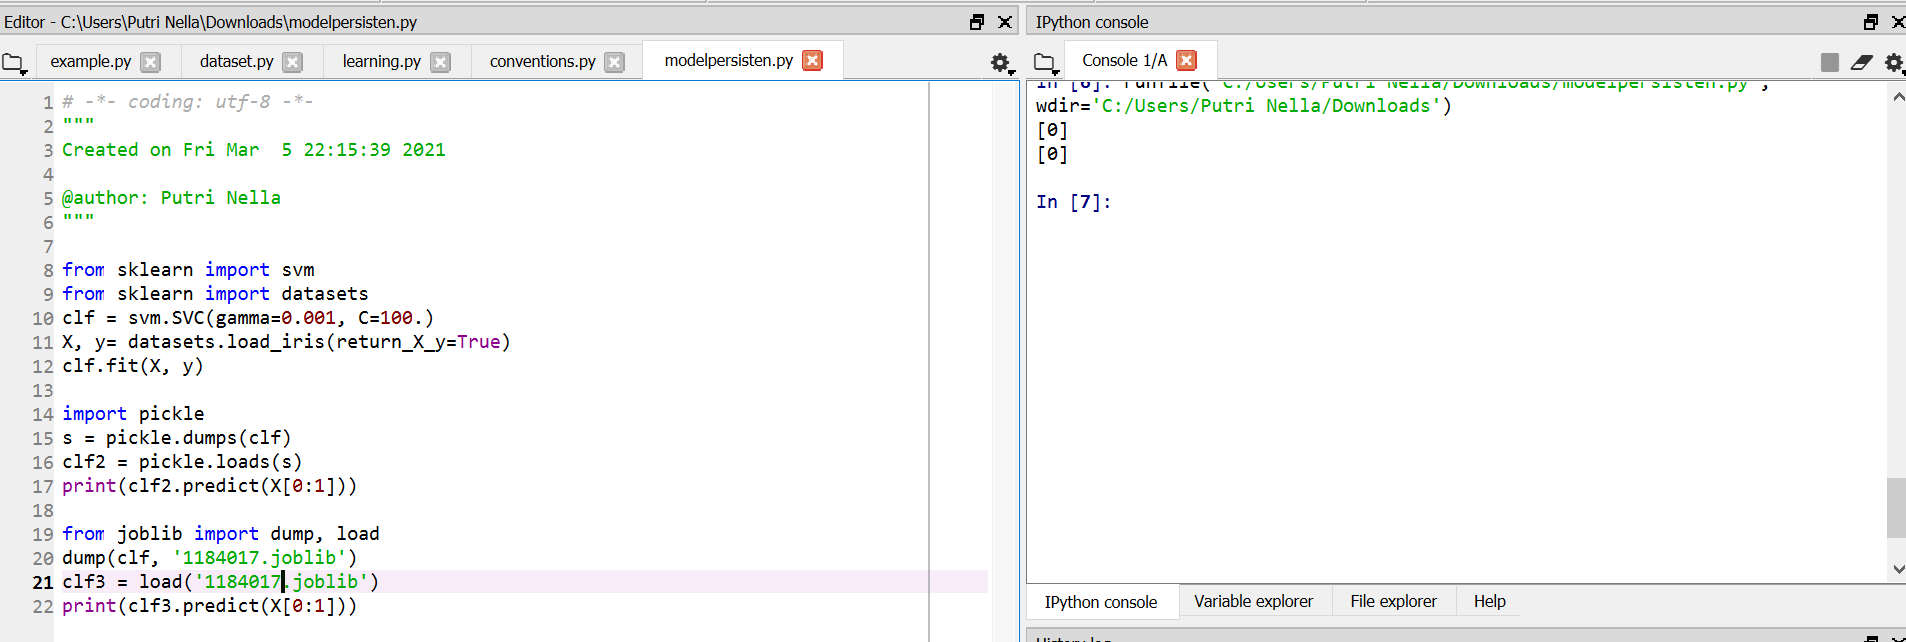
\includegraphics[width=.8\textwidth]{figures/1184017/chapter1/5.PNG}
    \end{center}
    \item Mencoba Conventions.
     \begin{center}
    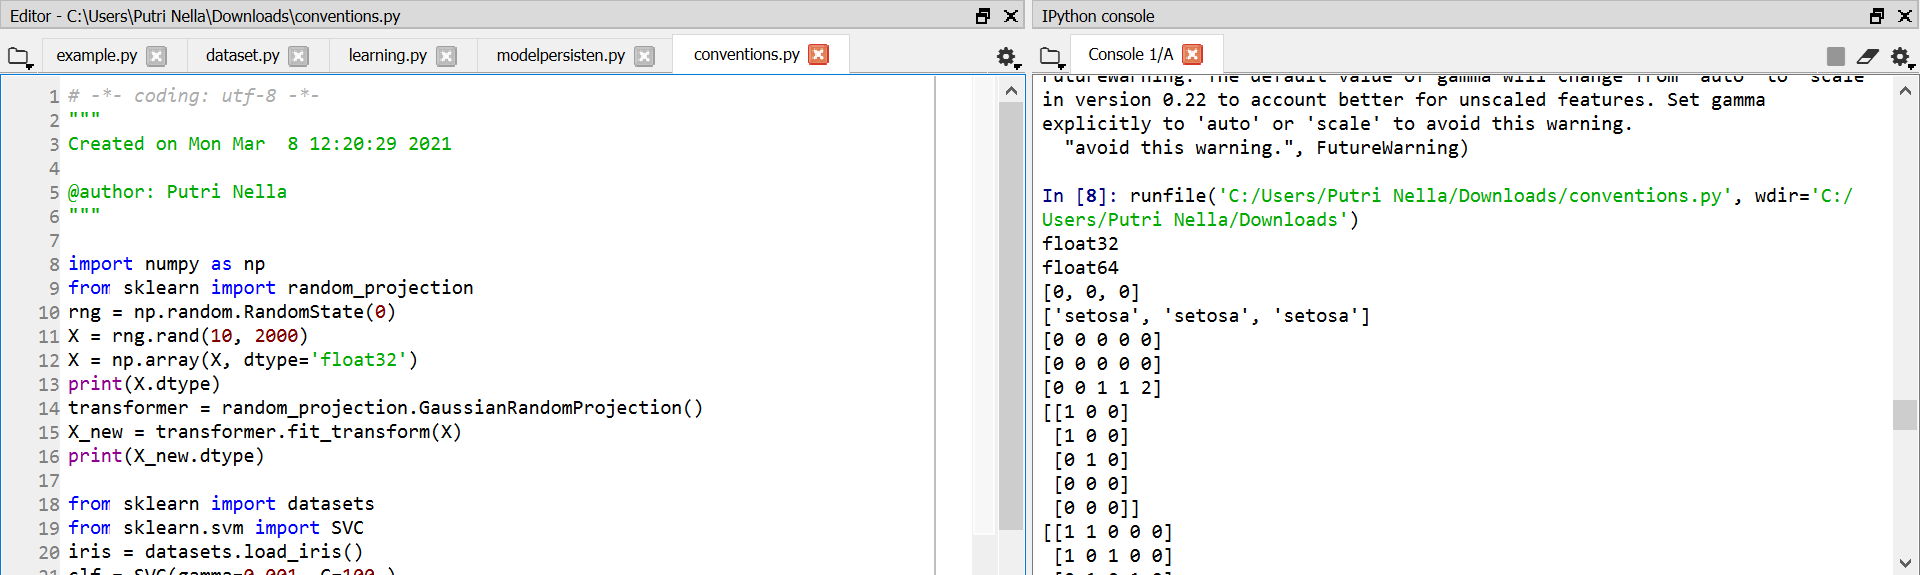
\includegraphics[width=.8\textwidth]{figures/1184017/chapter1/6.PNG}
    \end{center}
    \item Hasil Model persistence
     \begin{center}
    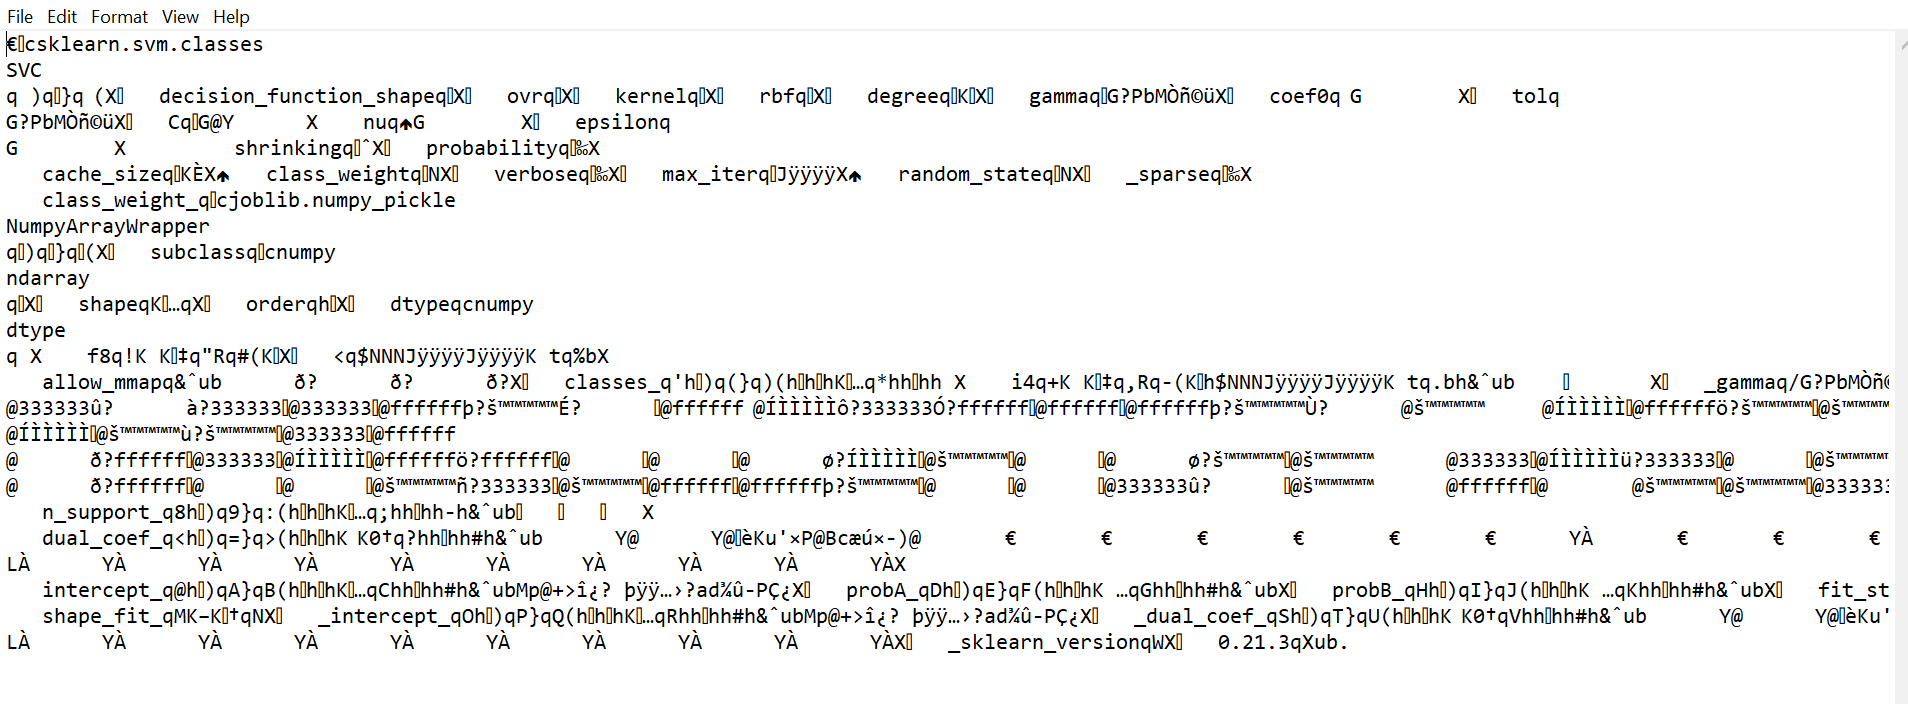
\includegraphics[width=.8\textwidth]{figures/1184017/chapter1/7.PNG}
    \end{center}
\end{enumerate}

\section{Error dan Penanganannya}
\begin{enumerate}
    \item Terdapat error dalam Dataset.py yaitu SyntaxError: invalid syntax
      \begin{center}
    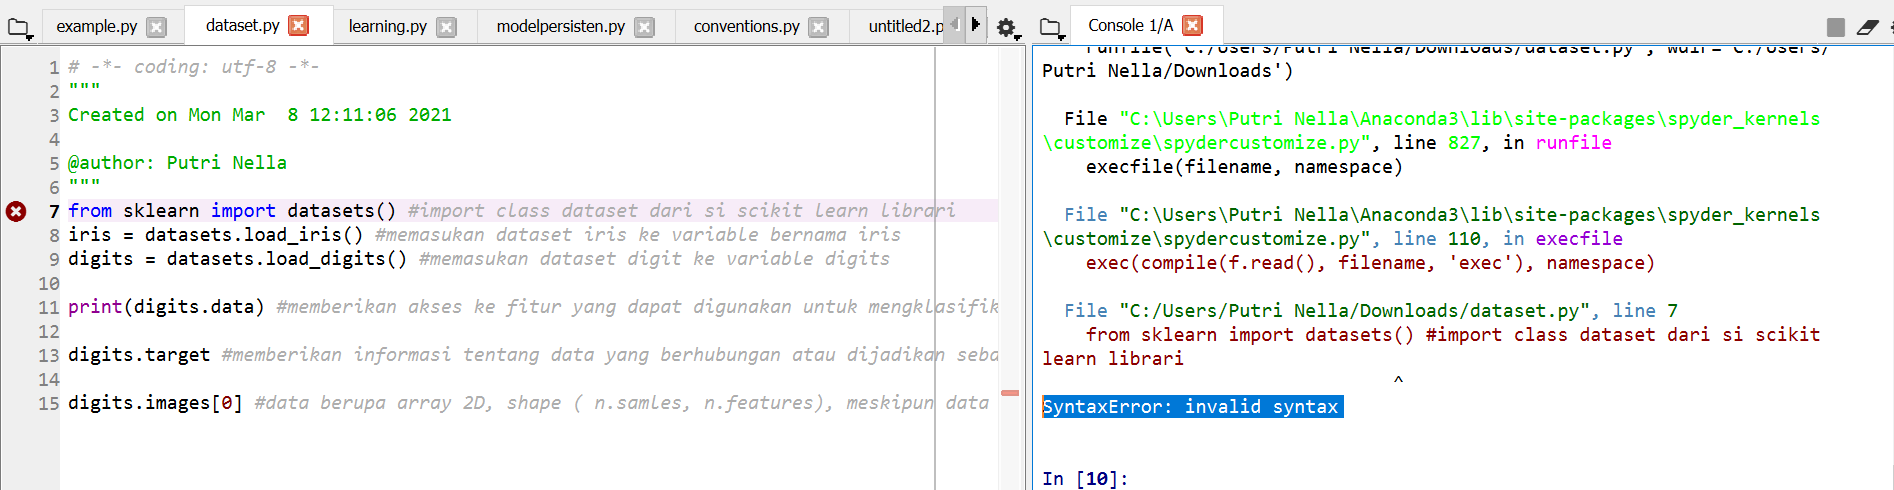
\includegraphics[width=.8\textwidth]{figures/1184017/chapter1/error1.PNG}
    \end{center}
    \\
    penangananya adalah harus menghapus tanda kurung disamping datasets.
     \begin{center}
    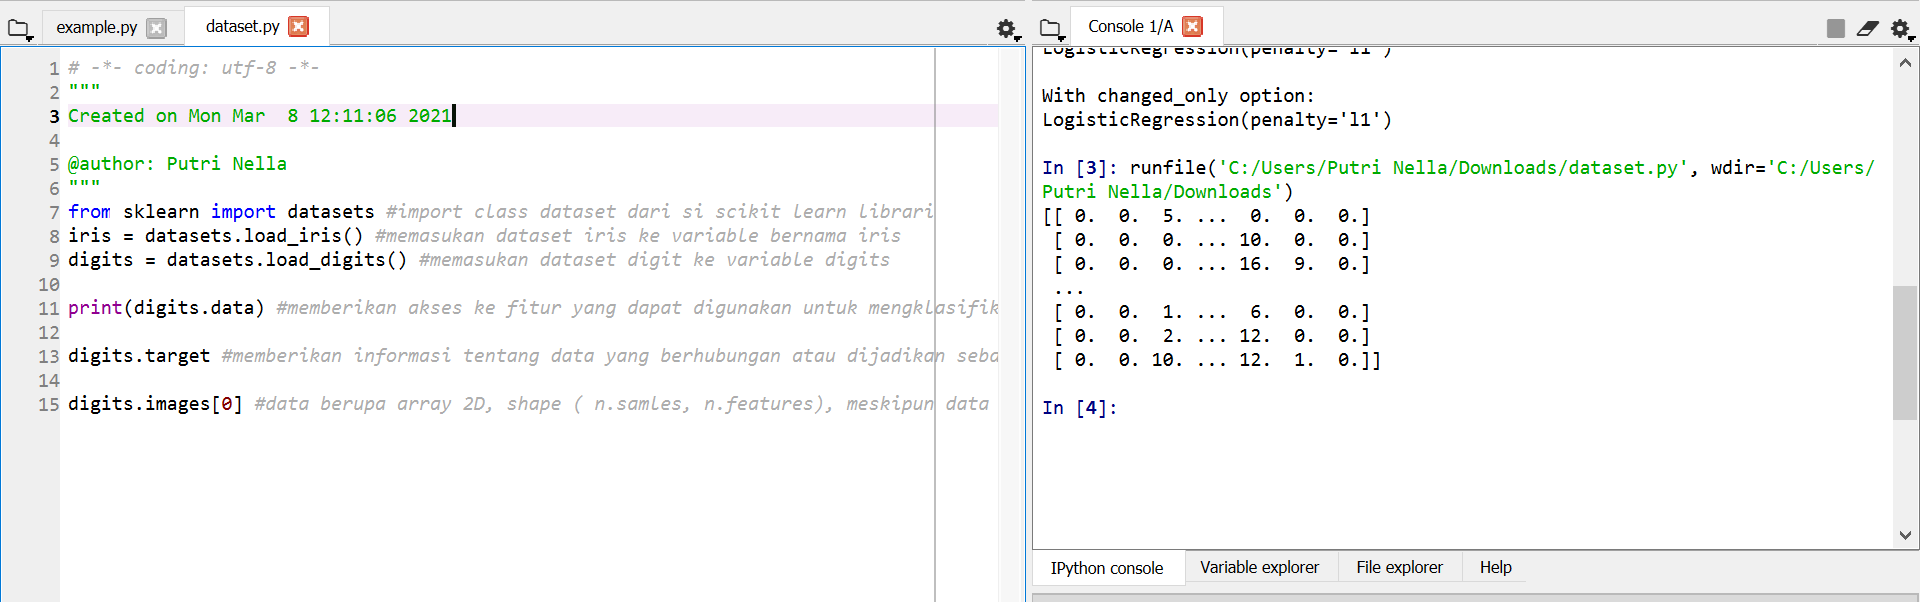
\includegraphics[width=.8\textwidth]{figures/1184017/chapter1/3.PNG}
    \end{center}
    \item Terdapat error dalam Modelpersisten.py yaitu ValueError: Found array with 0 sample(s) (shape=(0, 4)) while a minimum of 1 is required.
      \begin{center}
    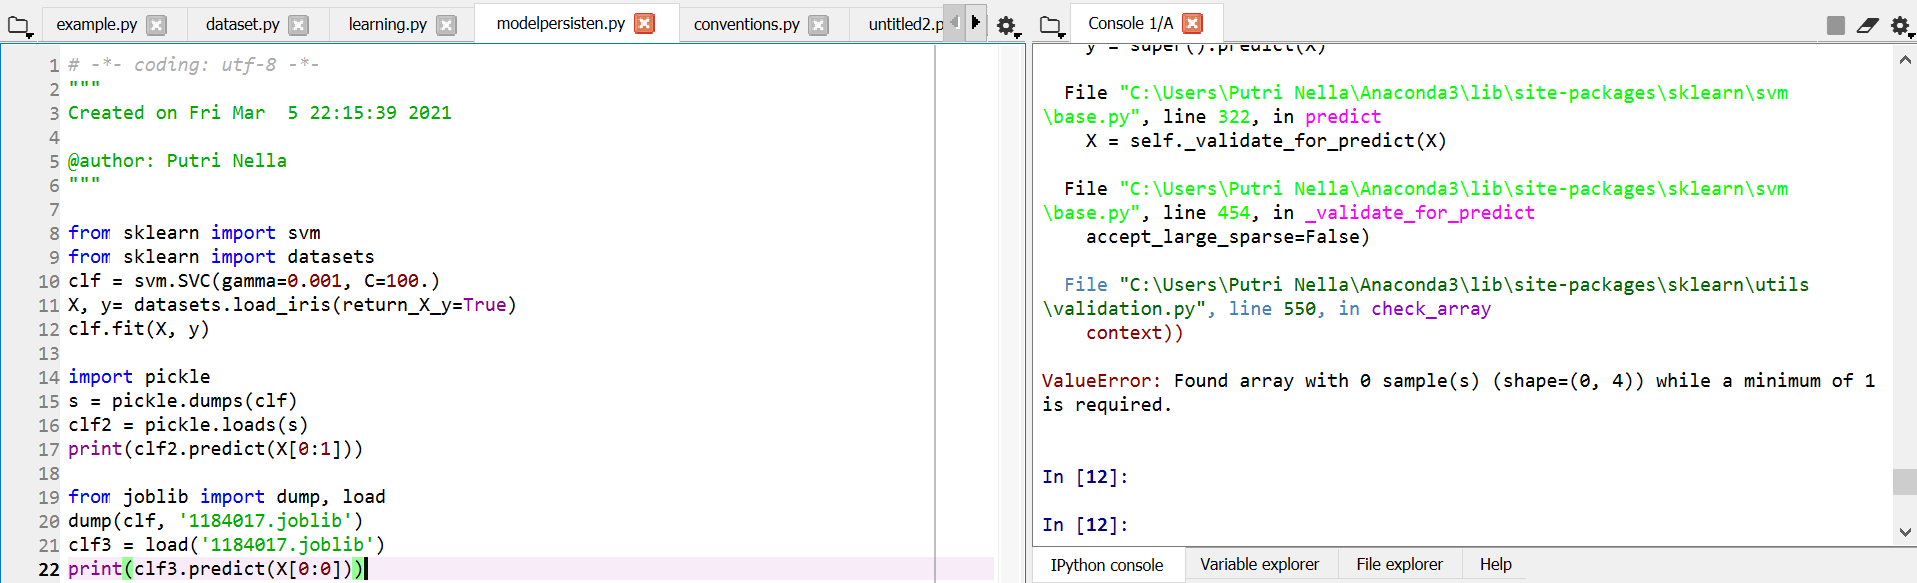
\includegraphics[width=.8\textwidth]{figures/1184017/chapter1/error2.PNG}
    \end{center}
    \\penangananya adalah harus mengubah value manjadi angka 1.
     \begin{center}
    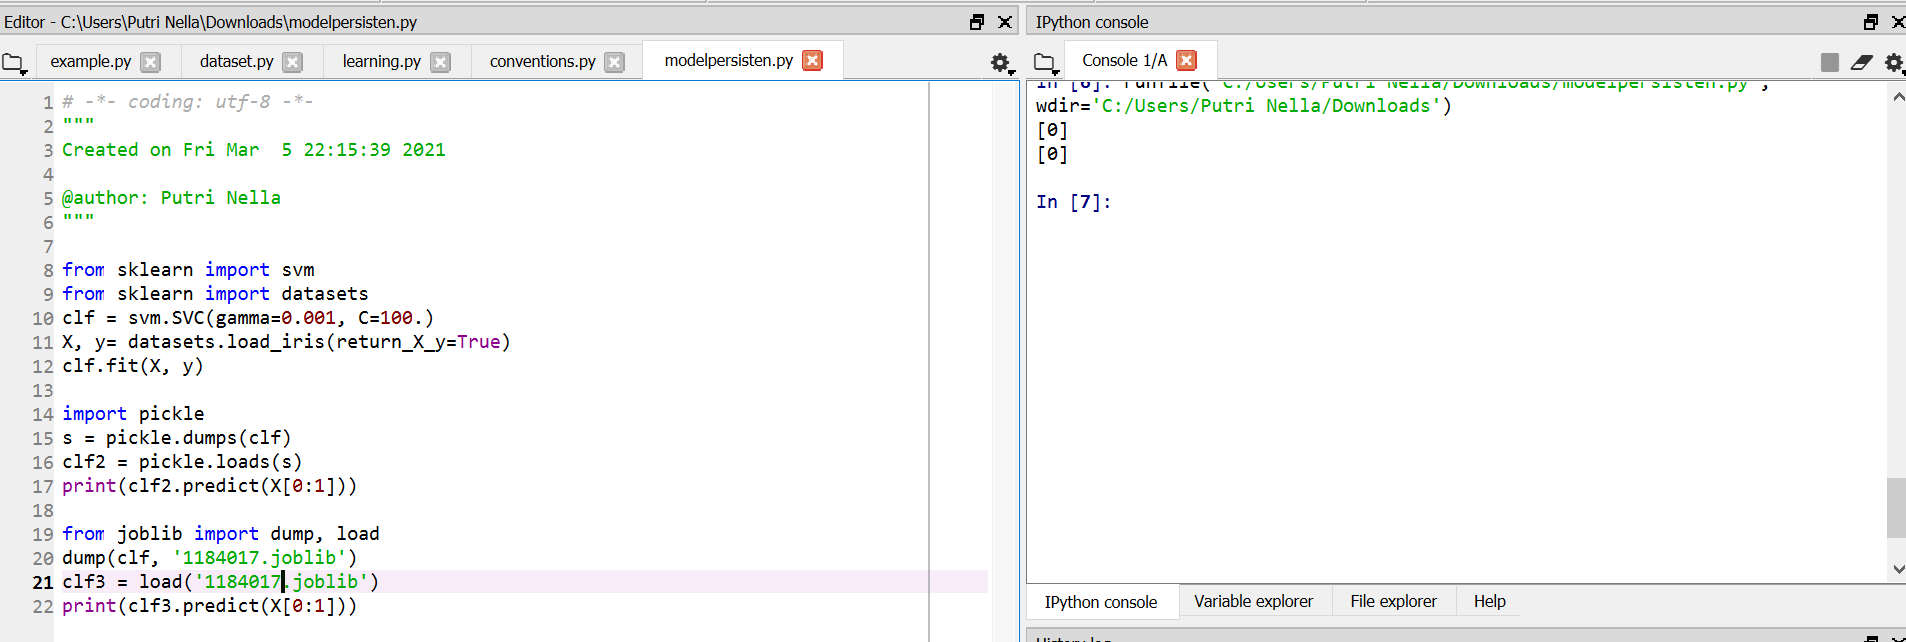
\includegraphics[width=.8\textwidth]{figures/1184017/chapter1/5.PNG}
    \end{center}

\end{enumerate}

